\chapter{Amélioration du projet}

%% 1) Gestion des évènements

%% 2) Dev client / serveur VNC pour intéragir directement depuis un ordinateur sur la liseuse 
%% Bref description de VNC
%% Utilisation de directvnc côté client ?
%% Serveur vnc côté liseuse
%% Schéma sur le fonctionnement

%% 3) Inclure ce client vnc à qemu

%% 4) Simulateur d'écran (plus besoin de passer par la liseuse)

\section{Gestion des événements}
La gestion des évènements, c'est à dire, être capable de détecter et de déclencher un traitement particulier lorsque l'utilisateur interagit avec la liseuse n'est pour l'instant pas implémenté.
\paragraph*{~}
Il semblerait que le driver utilisé pour l'écran de la liseuse ne prenne pas en compte les évènement de type \emph{touch}. D'après les recherches que nous avons pu faire, le driver TsLib serait meilleur pour la gestion de ces évènements.
\paragraph*{~}
Malheureusement, malgré des pistes pour la résolution de ce problème, nous n'avons pas assez de temps pour faire des recherches approfondies qui permettraient la mise en place d'une solution.


\section{Client / serveur VNC}

Un des objectifs pour améliorer le projet serait de développer un client et un serveur VNC. Le but étant de pouvoir contrôler directement la liseuse depuis un ordinateur.

\subsection{Description de VNC}

VNC est un système de visualisation et de contrôle d'un environ de bureau d'un périphérique distant (dans notre cas la liseuse). Ce système fonctionne via une communication client / serveur. Un serveur VNC doit être installé sur le périphérique à contrôler pour que un ou plusieurs clients s'y connectent. Le client VNC envoi au serveur différentes directives de mise à jour d'écran ou encore d'actions du clavier ou de la souris. Lorsque le serveur reçoit une directive, il met à jour son environnement graphique et le renvoi au client. Ces communications se font à travers un réseau en utilisant le protocole RFB.

\subsection{Côté serveur}

La serveur devra être installé sur la liseuse pour que celle-ci puisse partager son écran. Pour une utilisation optimal, il sera nécessaire de modifier le protocole RFB utilisé par le serveur VNC pour y inclure les événements de la liseuse (événement lors de l'appuie sur une zone de l'écran). Ce serveur va envoyer des directives à DirectFB qui fera ensuite la transition vers le matériel graphique pour modifier l'écran.

\subsection{Côté client}

Un programme client devra pouvoir se connecter au serveur présent sur la liseuse et envoyer des directives pour mettre à jour différentes zones de l'écran de la liseuse.

\begin{center}
	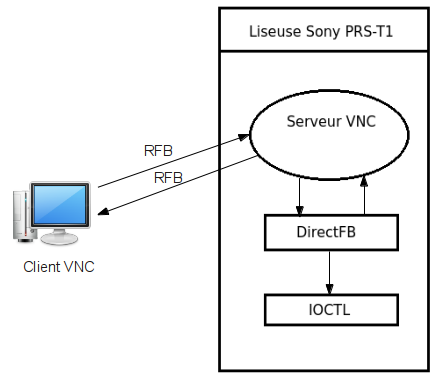
\includegraphics{VNCClientServeur.png}
\end{center}

\section{VNC et qemu}

Un autre point que l'on peut ajouter sur ce projet est d'intégrer VNC à qemu, cela afin que l'émulateur qemu puisse utiliser le serveur VNC installé sur la liseuse.


\section{Simulateur d'écran}

La dernière étape pour rendre le projet complet est de développer un simulateur d'écran de la liseuse. Pour cela il faut faire en sorte de gérer un affichage cohérent avec les temps de réponse de la liseuse Sony PRS-T1. C'est-à-dire que l'écran doit mettre un certain temps à se rafraîchir et pouvoir modifier seulement certaines zones de l'écran. De plus il faudrait y intégrer la gestion des événements, par exemple lors d'un clique souris simuler un appuie sur une zone de l'écran de la liseuse.

Enfin, une fois ce simulateur d'écran développé, l'objectif est de l'intégrer à qemu pour ne plus être dépendant de la liseuse. On aura alors un émulateur complet de la liseuse Sony PRS-T1.


%% A deplacer ...
\section{Protocol RFB}

RFB est un protocol simple pour l'accès à distance aux interfaces graphiques ds utilisateurs. C'est ce protocol qui est utilisé par VNC. Il y a d'un côté un visionneur, appelé client, et de l'autre côté un serveur qui va modifier le framebuffer afin de modifier l'affichage.

Le protocol RFB peut se décomposer en trois phases. Une première où le client et le serveur vont s'accorder sur la version du protocole à utiliser. Ensuite le client et le serveur vont s'envoyer des messages d'initialisation pour enfin pouvoir communiquer. A partir de ce moment, le client peut envoyer des demandes au serveur qui va lui retournera le résultat de cette requête.

\begin{center}
	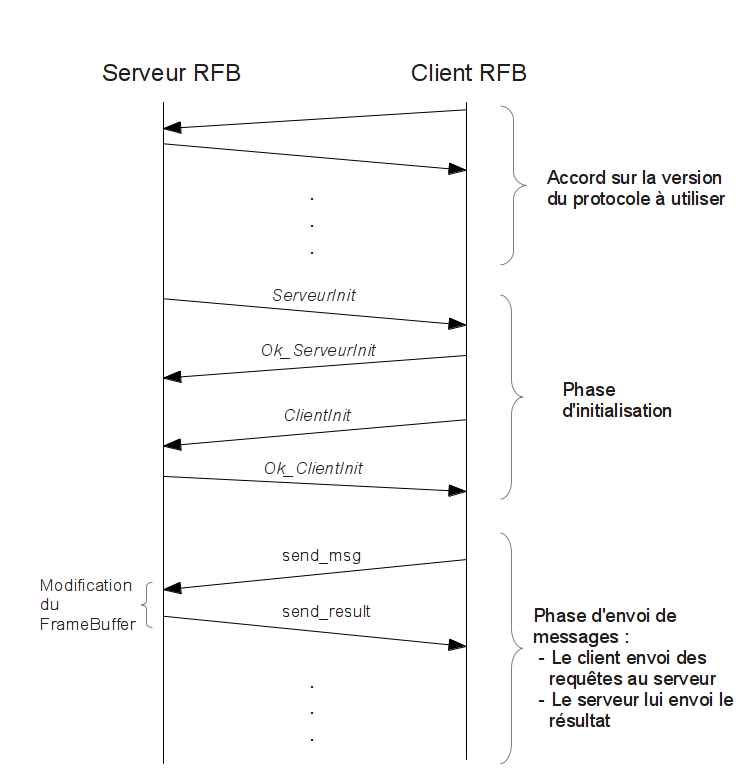
\includegraphics[scale=0.6]{RFBProtocol.png}
\end{center}